\documentclass [11pt, proquest] {uwthesis}[2020/02/24]

\usepackage{booktabs}% http://ctan.org/pkg/booktabs
\usepackage{array}
\usepackage{float}
\usepackage{graphicx}
\graphicspath{ {./images/} }

\setcounter{tocdepth}{1}  % Print the chapter and sections to the toc

\let\mffont=\sf

\begin{document}

\prelimpages

\Title{Securing WireGuard private keys with a hardware token\\}
\Author{Peter Van Eenoo}
\Year{2022}
\Program{Computer Science and Engineering}

\Chair{Brent Lagesse}{Dr.}{Computing \& Software Systems}
\Signature{William Erdly}
\Signature{Yang Peng}

\copyrightpage

\titlepage  


\setcounter{page}{-1}
\abstract{

WireGuard is a popular, secure, and relatively new VPN implementation that has seen widespread adoption. WireGuard's basic key management in the reference implementation leaves some weaknesses that could be exploited by threat actors to steal keys, compromising a user's identity or exploit their privilege. In my project I combined the industry-standard practice of isolating sensitive data with cutting-edge support for Curve25519 keys on select security keys. I created a WireGuard-compatible fork called WireGuard-HSM which uses the PKCS\#11 interface to securely access a user's private key and perform privileged operations on a USB security key. After performing two threat model analysis and comparing the results I show how my modifications improve the security of the system by decreasing the attack surface and mitigating two vulnerabilities if the host computer is compromised. WireGuard-HSMs security improvements are shown to come without a noticeable performance penalty.

}

\tableofcontents
\listoffigures

\chapter*{Glossary}      % starred form omits the `chapter x'
\addcontentsline{toc}{chapter}{Glossary}
\thispagestyle{plain}

\begin{glossary}

\item[WireGuard]

a VPN technology created in 2017 by Jason DonenFeld that operates at the network layer. It aims to be a replacement for popular TLS-based VPNs like OpenVPN and IPsec. WireGuard uses a fixed-set of cryptographic primitives and by design, has no support for negotiation of these primitives. 

\item[Curve25519]
an elliptic curve with a 256-bit key size. Designed by Daniel J. Bernstein in 2005\cite{bernstein_curve25519_2005}. 
Curve25519 has a digital signature algorithm named Ed25519 and a key derivation algorithm named X25519.

\item[X25519]
an algorithm that uses Curve25519 to implement Elliptic-curve Diffie–Hellman (ECDH) key exchange. This process is also known as a key derivation function (KDF). All KDF references refer specifically to X25519.

\item[AEAD]
Authenticated encryption with additional data. A class of encryption algorithms which enforce confidentiality and authenticity of data. 

\item[HKDF]
Hashed Message Authentication Code (HMAC)-based key derivation function. RFC5869 \cite{krawczyk_hmac-based_2010}

\item[AEAD]
Authenticated encryption with additional data. A class of encryption algorithms which enforce confidentiality and authenticity of data. 

\item[ChaCha20Poly1350]
an AEAD encryption algorithm which is composed of the ChaCha20 stream cipher and Poly1305 for message authentication code (MAC)

\item[PKCS\#11] a platform-independent interface standard for interacting with cyrptographic tokens governed by the OASIS technical committee\cite{noauthor_cryptsoft_2020}.
It defines a common interface for programs to interact with security keys, also referred to as cryptographic tokens.

\item[Hardware security module]
(HSM) is a dedicated, physical device that safeguards digital keys and provides limited-access to the resident keys for operations on messages such as encryption, decryption, verification and authentication. 

\item[Security Key]
a general term for a class of devices that implement a limited subset of HSM functionality. Security keys store cryptographic keys and restricts access through a limited interface. These devices typically connect to a computer or smartphone via USB or NFC and are small enough to be held on a user's key-ring.
Nitrokey Start\cite{noauthor_nitrokey_nodate} or YubiKey\cite{noauthor_discover_nodate}\cite{noauthor_u2f_nodate-1} are examples of such devices. 
I will use the terms Security key and HSM interchangeably.

\end{glossary}

\textpages

\chapter {Introduction} \label{introduction}

WireGuard is a new implementation of a Virtual Private Network (VPN) proposed in 2017. It has had a successful mainstream adoption, as evidenced by its recent inclusion in many open-source operating systems\cite{donenfeld_wireguard_nodate} as well as a native Windows kernel module\cite{noauthor_wireguard-nt_nodate}. MacOS, iOS, Android, FreeBSD and OpenBSD are supported as well.
WireGuard has been described as “crypto-opinionated”, meaning the protocol supports only one cryptographic primitive for each cryptographic requirement which allows it to completely forego cryptographic-protocol negotiation between peers, eliminating design complexity and reducing it's attack surface. 

For example, WireGuard only supports Curve25519 key-pairs for client authentication and key exchange, and ChaCha20Poly1350 for symmetric encryption\cite{donenfeld_wireguard_2017} of data.
Simplicity is a design goal of WireGuard, the core protocol is implemented in under 4,000 lines of code. WireGuard goes to great lengths to resist leaking any possible information about the connected peers; it encrypts the identity of the peers in the handshake process and no connection-state information is sent over the wire so peers mange the connection state themselves using a state machine. 

WireGuard has been shown to be very fast, out-performing IPsec and OpenVPN-based VPNs, in terms of throughput and response time\cite{donenfeld_performance_2018}, as well as easy to quickly port to a wide variety of operating systems. 

An important design simplification of WireGuard is the management of public and private keys. WireGuard does not use traditional x509 digital certificates or public key infrastructure. A peer's identity is anchored to a static Curve25519-based public key stored in the configuration file.
The static public keys of the initiator and responder must be pre-shared with both parties respectively, before a successful handshake can be made. 
A consequence of leaving key management up to the users is that this exposes a weakness in reference implementation of WireGuard, it's plain-text configuration file is an attractive target for threat actors.


\subsection{Problem Definition} \label{problem_definition}
After performing a threat model analysis of WireGuard, I identified local key handling as the primary weakness. In order address this problem, I looked at different ways to mitigate this weakness and decided to use an HSM. 


The key design goal of WireGuard-HSM is to the client's private key onto a USB-security key with cutting-edge support for Curve25519, while maintaining compatibility with mainline WireGuard clients. 
Another team of researchers have also identified WireGuard's handling as a weakness and we will briefly discuss their work on this topic in section \ref{related_work}.

\subsection{Goals}
In this project, my primary goal is to increase the security of WireGuard by improving it's key handling. I want to use well established methods in the computer security field to achieve this goal, without sacrificing compatibility. Instead of proposing compatibility-breaking changes, my secondary goal was to work within the confines of the existing protocol and maintain client compatibility, while improving security. I also wanted to understand what performance implications my design choices would impose on the system. System performance is discussed in section \ref{performance}

\subsection{Outline}
I will discuss WireGuard's authentication and identify mechanisms as well as the handshake process, in enough detail so readers can understand why my changes are relevant.
I will show how weaknesses in WireGuard's key management could lead to a threat actor compromising a private key and thereby a user's identity. 
I will briefly discuss what happens to the WireGuard system when a user's identify is compromised and why a threat actor might want to do this.
I will show how the security architecture design WireGuard-HSM safeguards a user's identity in the same scenarios.
Finally I will evaluate any performance impact of WireGuard-HSM on the system and the implications for usability.

\section {Contributions}
The Elliptic Curve, Curve25519 is being used in an increasing number of open-source and commercial products from SSH to Signal\cite{noauthor_things_2022}, however hardware support in 
security keys is currently almost non-existent. YubiKey is currently the most popular security key manufacturer, however all of their current products lack support for X25519. One of the goals of this project, as the first open source project to combine an X25519 supported security key with a popular open source VPN like WireGuard, will encourage more manufactures to add support for X25519 across the security key industry.

\section {Related-work}
\label{related_work}
The WireGuard handshake protocol has gone through extensive formal verification using Tamarin proof system \cite{donenfeld_formal_2018}. Researchers have identified some potential weaknesses in WireGuard around quantum computers\cite{hulsing_post-quantum_2021} but no serious vulnerabilities have been identified, since it was introduced five years ago in 2017.

WireGuard's key handling is a current area of research. A paper by \cite{wu_sewg_2020} focused on modifying WireGuard to use Trusted Execution Environment (TEE) of an Android phone to securely store the long-term static private key. The TEE is similar to the secure enclave in Intel processors. This work has the benefit that is supports a mobile operating system but it's implementation is restricted to a specific android maker's platform.

\section {Project scope}

My project is focused on improving WireGuard's handling of its private key.
It will be necessary to understand importance of the private key and how it's used during the WireGuard handshake process for authentication, when we discuss our threat model in section \ref{wg-ref-analysis}.


\chapter {Background}
\label{background}
So readers can understand the context of my project's modifications, we will discuss several key points about WireGuard's handshake process and it's components. Mainly how peers are authenticated, how the symmetric cipher is exchanged and how the handshake process works flows in general.

WireGuard's 'crypto-opinionated' design and lack of any negotiation does come with consequences. The lack of cryptographic negotiation means that if vulnerabilities are identified and a cryptographic component must be modified or replaced, this will result in complete peer incompatibility, until all peers are updated to the new protocol. 
This also means that project forks are limited in the scope of changes they can introduce, if they wish to maintain interoperability with mainline WireGuard peers.

WireGuard makes exclusive use of Curve25519 for user authentication and authorization. First I will discuss it's technical use in WireGuard and how it is tied to a users identity and authentication. For a complete description of the handshake process and details, see \cite{donenfeld_protocol_2018}\cite{donenfeld_wireguard_2017}.

\section{Curve25519 key pairs} \label{x25519}
Curve25519 is a patent-free, high-performance elliptic-curve with a reference implementation that is in the public-domain. This makes it an attractive curve for many projects \cite{noauthor_things_2022}.
A useful feature of Curve25519 is that any 32-byte value is a valid private key. Meaning no Curve25519 key requires validation which helps avoid small subgroup attacks. Curve25519 keys have also been shown to be immune to some classes of timing attacks\cite{noauthor_safecurves_2022}\cite{sasdrich_implementing_2015}.  Deriving the public key from the private key is fast enough that programs such as WireGuard don't need to store the client's public key in their configuration file. WireGuard only saves the private key and simply derives the public key on program start-up.

A user's identity is rooted in their Curve25519 'long-term static public key' which is generated from their private key and shared out-out-band with every peer that a user wishes to communicate.  
There are no mechanisms for key revocation built into the WireGuard protocol and the static public key never expires.

During the handshake process, WireGuard also creates short-lived Curve25519 key pairs which are independent of the long-term static public key. These short-lived key pairs are referred to as the ephemeral session keys and they used to derive the symmetric key to a peer during the handshake. 
Another important point is that these ephemeral session key-pairs are only valid for a default of 2 minutes per session. WireGuard has a novel key rotation mechanism which guarantees that nonce-reuse never happens but further discussion of this is out-of-scope for this paper. 



\section {Session Establishment}
\label{session_establish}
WireGuard assumes that each party's public key is securely exchanged out-of-band. This exchange must take place before a handshake can be performed. 
WireGuard refers to parties as an initiator and a responder, since there is no strict definition of client or server. A handshake is performed using an initiation message, sent by the initiator to the responder. The first packet is authenticated by including the peers encrypted public key in the initiation message, I will discuss this further in the next section.

This handshake has been described as a 1.5 round-trip-time (RTT) handshake over UDP which is inherently connection-less. See figure \ref{fig:simpleHandSeq} for a visual description. The 1.5 RTT handshake is defined by the following steps: the initiator sends a handshake initiation message, the peer responds to a properly authenticated initiation message with a handshake response message. Finally the initiator sends the first data packet. These three message are required for the session to be considered established and compose the 1.5 RTT handshake process. Consider the similarity to TCP's three-way-handshake.

\begin{figure}[ht]
\begin{center}
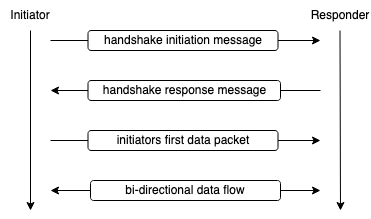
\includegraphics[width=10cm]{paper/images/handshake_process.png}
\caption{Simple Handshake Packet Sequence}
\label{fig:simpleHandSeq}
\end{center}
\end{figure}

\begin{figure}[ht]
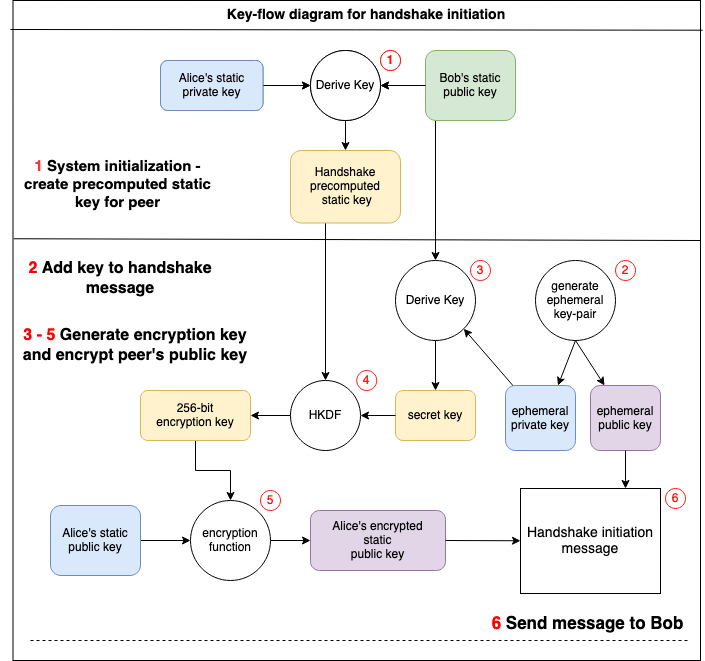
\includegraphics[width=15cm]{paper/images/key-flow-wg.png}
\caption{Detailed Handshake Initiation Process}
\label{fig:keyflow}
\end{figure}
\subsection{Handshake initiation}
\label{handinit}
Let's call the initiator Alice and the peer (the responder) Bob.
The diagram in \ref{fig:keyflow} shows the detailed process on Alice's computer that WireGuard goes through to send a handshake initiation message. First, WireGuard reads Alice's private key and Bob's public key from it's configuration file, sending them to a KDF to generate the handshake's precomputed-static key. Second, Alice generates an ephemeral Curve25519 key-pair and attaches that public key to her initiation message. The ephemeral private key and the precomputed static key from step 1, are used as input to an HKDF which generates, what WireGuard refers to as the chaining key. The chaining key is used in part as the key to symmetric-encryption function ChaCha20Poly1350 which encrypts Alice's static public key. The encrypted form of Alice's public key is finally added to the handshake initiation message and used by Bob to authenticate that only Alice could have sent this message.

When Bob receives this message, assuming he already has Alice's public key, he will follow this process in reverse-order. Bob will generate his own ephemeral key-pair and send his ephemeral public key in his handshake response message to Alice. The chaining key mentioned earlier is also used as input into an HMAC function, so both parties can derive the sending and receiving keys for symmetric encryption of transport data.
The state is now identical for both peers and they have each derived the the symmetric encryption key to decrypt data sent by the peer. It's worth noting that unlike many encryption schemes, the key to the symmetric cipher is not same in each direction because each peer chooses their own 'sending channel' cipher-key.

A benefit of requiring that the sender include their encrypted public key, is that any party running WireGuard is resistant to active network enumeration. In order to elicit a response from a node running WireGuard, the initiator must have knowledge of the responder's public key and the responder must have knowledge of the initiators public key.

WireGuard uses encrypted timestamps to avoid replay attacks and it employs a novel cookie mechanism to avoid DoS attacks by unauthenticated parties however further discussion on the handshake is out of scope for this paper.

\subsubsection{Key Rotation}
\label{keyrotate}
WireGuard sessions guarantee perfect forward secrecy by including a key rotation process (rekey) between peers. This rekey event occurs after a default of 120 seconds, or after 2\textsuperscript{60} messages have been exchanged. The key rotation process is essentially another handshake process with one key difference: if Alice is the peer performing the rekey process, then in step 1, see figure \ref{fig:keyflow}, Bob's most recent ephemeral public key is used as input to the KDF instead of his static public key. This has implications for my project which we will discuss in section \ref{pk_design}

The WireGuard protocol has no distinction between authentication and authorization. If a peer can successfully authenticate a handshake initiation message and response, then the user is allowed to freely communicate over the session, with whatever resources may be gated on or behind the WireGuard peer.
Now that we understand the handshake initiation process and session key rotation in more detail, it should be clear how the initiators static private and public key, as well as the responders public key, form the basis for establishing a WireGuard session.

\begin{figure}[ht]
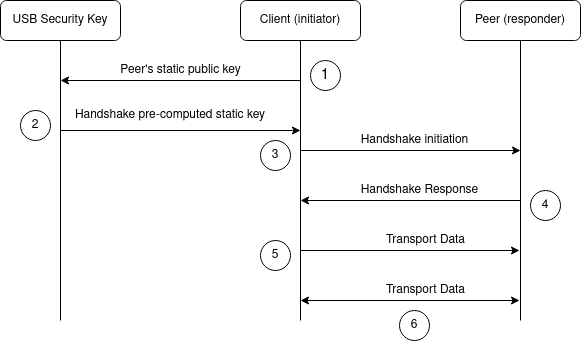
\includegraphics[width=6cm]{paper/images/Process_Diagram.png}
\caption{Informal Handshake Narration Process}
\label{fig:handshake_process}
\end{figure}

\subsection {Identity and Authentication}
\label{identity}

\begin{figure}[ht]
\frame{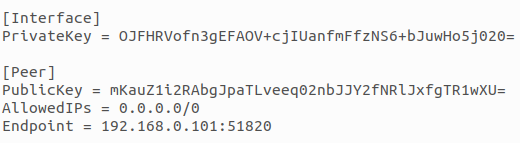
\includegraphics[width=12cm]{paper/images/wg_config.png}}
\caption{Example WireGuard Configuration File from the Reference Implementation}
\label{fig:wg_config}
\end{figure}

\section{Key Storage}
As mentioned previously, WireGuard leaves key management up to the user.
Figure \ref{fig:wg_config} shows an example configuration file for WireGuard. The user's private, long-term static private key is under the "[Interface]" section and "[Peer]" section contains each peer's pre-shared static public key, as well as internet address information.

WireGuard saves a user's private key as Base64 encoded plain-text in the configuration file. There is no support for adding a password to a private key or support for traditional digital certificates. Even Curve25519 keys generated by OpenSSL are not compatible with WireGuard, unless the ANS.1 header is stripped from it's output.

\section{Nitrokey and HSMs}
An HSM is a widely used, industry-standard device that is used to safeguard digital keys. Many HSMs undergo rigorous testing and certification, to validate their compliance with internationally recognized standards such as Federal Information Processing Standard (FIPS) and Common Criteria. They also typically use the ubiquitous and platform-independent PKCS\#11 interface. 

At the time of writing, the only commercially available HSM that offered the right features features for the project was the "Nitrokey Start" from Nitrokey in Germany\cite{noauthor_nitrokey_2022}. A few HSM list support for 'Curve25519' yet most only support Ed25519 while WireGuard only uses the X25519 algorithm of Curve25519.

The Nitrokey Start connects to the computer via a USB-A interface. It securely stores cryptographic keys and provides an interface using the PKCS\#11 standard.
An HSM safeguards private keys by only allowing authenticated users to perform a strict subset of key management and cryptographic functions on a slot. A slot holds private and public keys and is protected by a user pin. HSMs are also designed in such a way that physical tamping with the device should destroy the private-keys, making them unreadable and useless. 
\begin{figure}[ht]
\frame{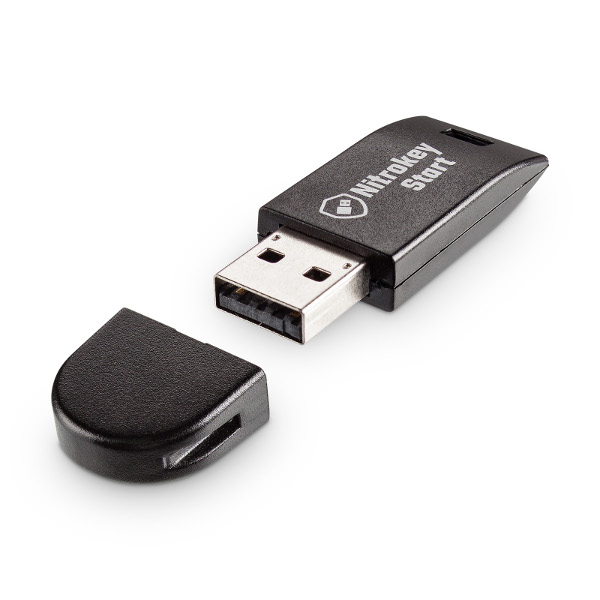
\includegraphics[width=6cm]{paper/images/nitrokey.jpg}}
\caption{Image of the Nitrokey Start Hardware Security Module}
\label{img:nitrokey}
\end{figure}

\chapter {Methodology}
Here I discuss key parts of the project architecture, so readers can understand the context of the different systems that were created for my project.

The confidentiality of a user's private key is paramount to proper client authentication and authorization in WireGuard. My project WireGuard-HSM, aims to improve upon WireGuard's key handing by using an HSM to securely store the private key, without modifying WireGuard in such a way to introduce incompatibility.

\section{Project Design}
\begin{figure}[ht]
\begin{center}
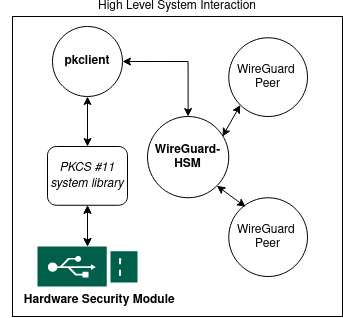
\includegraphics[width=8cm]{paper/images/high-level-overview.png}
\caption{A High-Level WireGuard-HSM System Interaction Diagram}
\label{fig:highlevel_system}
\end{center}
\end{figure}

Figure \ref{fig:highlevel_system} shows the major WireGuard-HSM system interaction. When WireGuard-HSM attempts to establish a new session with a peer, WireGuard-HSM interacts with a module named 'pkclient' which uses the PKCS\#11 interface to talk to a connected HSM. 

\subsection{Pkclient}
\label{pk_design}
I created a standalone project called 'pkclient' to handle the interactions with the HSM and manage state. Pkclient implements functions specific to the cryptographic operations required by WireGuard but it's implemented as a standalone module to limit the required modifications to WireGuard. Pkclient itself incorporates a golang package to integrate the low-level PKCS\#11 interface calls, exposing a simplified interface to callers.  Pkclient handles the HSM session establishment, verification that the correct key-types are present on the HSM, user-interactions for pin authentication. 
From WireGuard-HSM's point of view, pkclient is responsible for key derivation functions when the long-term static private key is needed as input, which is performed inside the HSM. When the peer session expires and performs the key rotation, described in section \ref{keyrotate}, the ephemeral public key of the peer is sent in a call to pkclient to derive the session's new shared secret. 

Normally WireGuard has full-access to the long-term static private key for deriving the long-term static public key, so pkclient must also provide a function to return the public key contents, which enables the user to share their public key with other peers.


\subsection{WireGuard-HSM}
WireGuard-HSM has the long-term private static key completely absent from the configuration file, replaced by a system library path to a PKCS\#11 library and the slot number on the HSM to use, see an example file in section \ref{fig:wg_hsm_config}.  In places where WireGuard expects access to the private key, changes were made to use the interface with pkclient for those calls instead.

WireGuard-HSM was designed to work in a two modes, the HSM mode and the original software mode. 
The 'software mode' is the original, unchanged mode that has access to the private key in the configuration file. WireGuard-HSM executes it's program flow in the same way as WireGuard-go but it used if/else statements to access the HSM or software mode. This approach helped me ensure that no incompatibility was introduced into the system. 

Simplicity and separation of privileges were primary goals in my system design so by design WireGuard-HSM abstracts much of it's functionality over to pkclient, keeping the changes to the WireGuard-go code-base to a minimum. 

Some small changes were made to the 'wireguard-tools' package to allow me to modify the configuration file for WireGuard-HSM but they out of scope for our purposes and only affect program initialization.

\begin{figure}[ht]
\frame{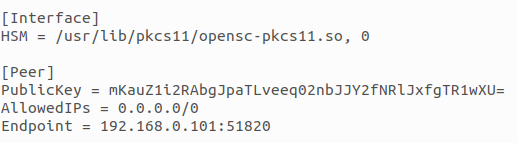
\includegraphics[width=12cm]{paper/images/wg-hsm_config.png}}
\caption{Example WireGuard-HSM Configuration File}
\label{fig:wg_hsm_config}
\end{figure}

\section{Threat Model}
Since WireGuard and all VPN clients, allow users access to protected resources across networks, there is inherent value for an attacker to gain access to these systems.
The attacker may be highly motivated, targeting a specific individual or the attacker may be opportunistic, deploying malware en-mass and harvesting credentials of WireGuard nodes, for later sale or use.


In the following section, I discuss the threat models for WireGuard and WireGuard-HSM, comparing WireGuard-HSM to see the relative strengths and weaknesses. This will help us evaluate the system design and perform a comparative threat model analysis. This analysis will show the relative strengths and weaknesses of the designs and if WireGuard-HSM has improved the security of the system at all.

\section{Threat Model Layout}
In order to assess risk in both systems, I will identify and calculate the risk for a given weakness based upon the DREAD model. I will use the rankings and descriptions of risk by following OpenStack Security Group's use of the DREAD and OWASP \cite{noauthor_securityossa-metrics_2022}\cite{noauthor_threat_2022}. The five categories are defined as follows:

\begin{itemize}
  \item \textbf{D}amage - how high is the impact of a successful attack?
  \item \textbf{R}eproducibility - how easy it is to reproduce the attack? 
  \item \textbf{E}xploitability - how easy is it to launch the attack?
  \item \textbf{A}ffected users - how many people will be impacted?
  \item \textbf{D}iscoverability - how easy it is to discover the threat?
\end{itemize}

\label{dread}
DREAD scores are criticized as being subjective, however the calculated risk score can help us identify the relative strength and weaknesses when applied to similar systems. The scores are based on a ranking of 1-10, low to high for each category, added together and divided by the number of categories to give a final score to the weakness. The calculation of risk is as follows:

"Risk = (DAMAGE + REPRODUCIBILITY + EXPLOITABILITY + AFFECTED USERS + DISCOVERABILITY) / 5"
I will use also use Threat Model Data-Flow Diagrams to identify where data flows across trust boundaries.
I will classify vulnerabilities and mitigations using terminology from the STRIDE method\cite{hernan_uncover_2019}.

\chapter {Threat Models and Comparison}
The two threat models in the following sections are primarily concerned with how data at rest is handled by both systems. WireGuard's handling of data in transit is out of scope for the analysis.
First I will identify and evaluate the risks in the WireGuard reference implementation. Second I will identify and evaluate the same risks and any new risks in WireGuard-HSM. Finally I will compare the results to draw my conclusions about the modifications in WireGuard-HSM.

\section {WireGuard - Reference Implementation}
\label{wg-ref-analysis}
This threat model is focused on WireGuard's: 1. Asset handling related to configuration file which contains private and public keys. 2. The security controls around the assets. 3. The threats to the system. 
The computer running WireGuard will be considered Alice's computer and the WireGuard peer that Alice connects to is Bob. Both computers are turned on and connected to the network but Alice has not yet established a WireGuard session to Bob's computer. Refer back to section \ref{handinit} on how WireGuard establishes a session with a peer. 

\begin{figure}[ht]
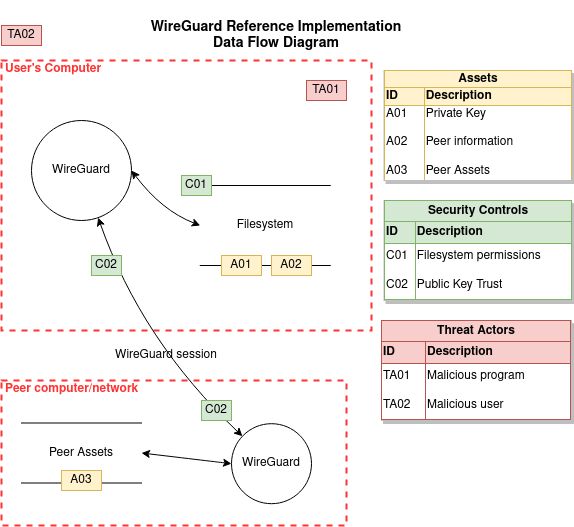
\includegraphics[width=14cm]{paper/images/WGH_DFD.png}
\caption{Threat Model for the WireGuard Reference Implementation - Data Flow Diagram}
\label{fig:wg_ref_dfd}
\end{figure}

\subsection{Assets}
The file system on Alice's computer contains the WireGuard configuration file \ref{fig:wg_config}. 
Asset A01 is Alice's Curve25519-based long-term static private key. Asset A02 is Bob's connection information consisting of his static public key and internet address. 
Asset 03 is the label for any potential assets on Bob's side of the WireGuard tunnel. Access to Bob's machine might be a highly valuable asset or Bob's network access might be the highly valuable asset. This model combines these possibilities into 'Peer Assets' for simplification.

\subsection{Security controls}
Access control in WireGuard's reference implementation for A01 and A02 is C01: file system permissions. Most of the documentation indicates that sufficient file-system permissions' should be set on the WireGuard configuration file to allow only administrator access and restrict access by unprivileged users. This is not an enforced measure, meaning WireGuard will still start and not warn the user if the file permissions are insufficient. 

Security control C02, access to each WireGuard peer, is the pre-shared public key system implemented by WireGuard.

\section{Threat Actor 1}
The primary threat is TA01: a piece of malware that has gained access to Alice's computer and will search for keys in configuration files. This malware could have been delivered by acquiring a zero-day exploit or by using a known vulnerability with a piece of software running on Alice's computer. Using a known vulnerability would likely lower the cost of the attack.

\subsection{Insufficient permissions}
If TA01 gains access to Alice's computer and the file system permissions were not correctly set on the WireGuard configuration file, then the threat gains access to A01 and A02. Access to these assets results in loss of A03 by bypassing C02. 
See table \ref{attack1-ref} and \ref{attack3-ref}.

\subsection{Sufficient permissions}
If C01 is configured properly, then TA01 will need exploit one more vulnerability, in-order to gain access to A01 and A02. This offers a single layer of security, so the cost of this attack cost is slightly higher. Exploit chains are common-place in today's attacks so this is considered a reasonable assumption.  
See table \ref{attack2-ref} and \ref{attack4-ref}.

\section{Threat Actor 2}
TA02 is a malicious user who gains direct or indirect access to Alice's computer.  

In a direct method of attack, TA02 gains physical access to Alice's laptop and uses some technical or non-technical exploit to read the hard-drive. If Alice's machine uses disk-encryption then this increases the difficulty of the exploit because a second exploit must be used to read the disk contents.
See table \ref{attack5-ref} and \ref{attack6-ref}.

The indirect method of attack could be performed by TA02 using social engineering tactics such as a phone-call or email, masquerading as someone from Alice's IT department, asking her to, in some way, disclose the contents of the WireGuard configuration file, leading to disclosure of assets A01 and A02.
See table \ref{attack7-ref} 

\section{Vulnerabilities}
Once any of the previously weaknesses and have been taken advantage of by a threat, and the threat actor gains access to assets A01 and A02, this creates two classes of vulnerabilities in our WireGuard system.

\subsection{Spoofing}
\label{spoofing}
Loss of A01 and A02 together allow an attacker to spoof Alice's identity with Bob because the attacker can complete a handshake with Bob as Alice and establish an authenticated session. VPN's are commonly used as the first layer of defense for network access, so A03 is an attractive asset.
In this scenario, spoofing threatens authentication in our system between because unauthorized parties can now masquerade as authorized users, potentially gaining access to protected resources. 

\subsection{Denial of Service}
\label{dos}
A Denial of Service vulnerability is also possible with the loss of A01 and A02. Once a threat can perform the impersonation of Alice, then a DoS could be leveraged against any future connection attempts that Alice's may perform with Bob. When Bob receives and establishes a session with Alice's credentials, the initiator includes a randomly generated 4-byte value as the 'sender's index'. Subsequent handshake initiation messages must include this value or the receiver will drop the packet. Once Bob has an established session with the threat, the real Alice's initiation messages won't have the correct, random sender's index according to Bob's session table and he will drop her packets.

A DoS attack threatens availability in the system because Alice's connection to Bob's resources can be denied by a malicious third-party.

\subsection{Attack Tables}
\begin{table}[H]
\label{attack1-ref}
\begin{tabular}{|m{3cm}|m{.9cm}|p{27em} |}
\multicolumn{3}{l}{Potential for: Information Disclosure, Spoofing, DoS}                   \\
\hline
Category & Score & Rationale                                                    \\
\hline
Damage          & 9     & Loss of A01, A02, A03. DoS for a single user possible            \\
\hline
Reproducibility & 6     & Two steps required, tooling and scripting readily available    \\
\hline
Exploitability & 5      & Exploit is available/understood, usable with only moderate skill by authenticated users or malware \\
\hline
Affected users  & 5     & At least two users are affected                     \\
\hline
Discoverability & 5     & Attack may be targeted - exploited by general malware infection \\
\hline
\multicolumn{3}{l}{\textbf{Dread Score: 6}} 
\end{tabular}
\caption{Attack 1 - Loss of A01 and A02 after access to configuration file by using malware delivered using a known vulnerability and the configuration file permissions are incorrectly set}
\end{table}

\begin{table}[H]
\label{attack2-ref}
\begin{tabular}{|m{3cm}|m{.9cm}|p{27em} |}
\multicolumn{3}{l}{Potential for: Information Disclosure, Spoofing, DoS}                   \\
\hline
Category & Score & Rationale \\
\hline
Damage          & 9     & Loss of A01, A02, A03. DoS for a single user possible            \\
\hline
Reproducibility & 5     & Three steps required, tooling and scripting readily available    \\
\hline
Exploitability & 5      & Exploit is available/understood, usable with only moderate skill by authenticated users or malware \\
\hline
Affected users  & 5     & At least two users are affected                      \\
\hline
Discoverability & 4     & Attack may be targeted - exploited by general malware infection \\
\hline
\multicolumn{3}{l}{\textbf{Dread Score: 5.6}} 
\end{tabular}
\caption{Attack 2 - Loss of A01 and A02 after access to configuration file by using malware delivered using a known vulnerability and the configuration file permissions are correctly set}
\end{table}

\begin{table}[H]
\label{attack3-ref}
\begin{tabular}{|m{3cm}|m{.9cm}|p{27em} |}
\multicolumn{3}{l}{Potential for: Information Disclosure, Spoofing, DoS}                   \\
\hline
Category & Score & Rationale \\
\hline
Damage          & 9     & Loss of A01, A02, A03. DoS for a single user possible            \\
\hline
Reproducibility & 4     & Two steps required, tooling and scripting readily available    \\
\hline
Exploitability & 4      & Advanced techniques required. General malware infection would have unimpeded access to access assets  \\
\hline
Affected users  & 5     & At least two users are affected                      \\
\hline
Discoverability & 4     & Attack may be targeted - exploited by advanced malware \\
\hline
\multicolumn{3}{l}{\textbf{Dread Score: 5.2}} 
\end{tabular}
\caption{Attack 3 - Loss of A01 and A02 after access to configuration file by using malware delivered using a zero-day exploit and the configuration file permissions are incorrectly set}
\end{table}

\begin{table}[H]
\label{attack4-ref}
\begin{tabular}{|m{3cm}|m{.9cm}|p{27em} |}
\multicolumn{3}{l}{Potential for: Information Disclosure, Spoofing, DoS}                   \\
\hline
Category & Score & Rationale \\
\hline
Damage          & 9     & Loss of A01, A02, A03. DoS for a single user possible            \\
\hline
Reproducibility & 3     & Two steps required, tooling and scripting readily available    \\
\hline
Exploitability & 3      & Advanced techniques required. General malware infection would have unimpeded access to access assets  \\
\hline
Affected users  & 5     & At least two users are affected                      \\
\hline
Discoverability & 3     & Attack may be targeted - exploited by advanced malware \\
\hline
\multicolumn{3}{l}{\textbf{Dread Score: 4.6}} 
\end{tabular}
\caption{Attack 4 - Loss of A01 and A02 after access to configuration file by using malware delivered using a zero-day exploit and the configuration file permissions are correctly set}
\end{table}

\begin{table}[H]
\label{attack5-ref}
\begin{tabular}{|m{3cm}|m{.9cm}|p{27em} |}
\multicolumn{3}{l}{Potential for: Information Disclosure, Spoofing, DoS}                   \\
\hline
Category & Score & Rationale \\
\hline
Damage          & 9     & Loss of A01, A02, A03. DoS for a single user possible            \\
\hline
Reproducibility & 4     & Two steps required. Attacker must gain physical access to the computer     \\
\hline
Exploitability & 7      & Exploit is understood, usable by unskilled attacker \\
\hline
Affected users  & 5     & At least two users are affected                      \\
\hline
Discoverability & 3     & Attack must be targeted to user \\
\hline
\multicolumn{3}{l}{\textbf{Dread Score: 5.6}} 
\end{tabular}
\caption{Attack 5 - Loss of A01 and A02 after access to configuration file by using physical access to unprotected machine.}
\end{table}

\begin{table}[H]
\label{attack6-ref}
\begin{tabular}{|m{3cm}|m{.9cm}|p{27em} |}
\multicolumn{3}{l}{Potential for: Information Disclosure, Spoofing, DoS}                   \\
\hline
Category & Score & Rationale \\
\hline
Damage          & 9     & Loss of A01, A02, A03. DoS for a single user possible            \\
\hline
Reproducibility & 4     & Two steps required. Attacker must gain physical access to the computer     \\
\hline
Exploitability & 5      & Exploit is understood, usable by moderately skilled attacker  \\
\hline
Affected users  & 5     & At least two users are affected                      \\
\hline
Discoverability & 3     & Attack must be targeted to user \\
\hline
\multicolumn{3}{l}{\textbf{Dread Score: 5.2}} 
\end{tabular}
\caption{Attack 6 - Loss of A01 and A02 after access to configuration file by using physical access to a protected machine.}
\end{table}

\begin{table}[H]
\label{attack7-ref}
\begin{tabular}{|m{3cm}|m{.9cm}|p{27em} |}
\multicolumn{3}{l}{Potential for: Information Disclosure, Spoofing, DoS}                   \\
\hline
Category & Score & Rationale \\
\hline
Damage          & 9     & Loss of A01, A02, A03. DoS for a single user possible            \\
\hline
Reproducibility & 4     & Two steps required. Attacker must find and convince user to disclose contents of configuration file    \\
\hline
Exploitability & 5      & Little technical knowledge is required but trust or deception must be used   \\
\hline
Affected users  & 5     & At least two users are affected                      \\
\hline
Discoverability & 3     & Attack is well understood  \\
\hline
\multicolumn{3}{l}{\textbf{Dread Score: 6.6}} 
\end{tabular}
\caption{Attack 7 - Loss of A01 and A02 after access to configuration file is gained by social engineering.}
\end{table}


\section{Vulnerability Mitigation}
\label{vulns}
Both of the vulnerabilities that were identified, spoofing and DoS, were only enabled once the system suffered an information disclosure of the plain-text configuration file. We can address the root of both vulnerabilities by applying STRIDE's recommended mitigation for information disclosure which is confidentiality. 

The confidentiality of the configuration file is a weakness in the design of the system. The entire configuration file cannot be p
Security is often a series of trade-offs, in which system designers must consider user-convenience vs system security. If I remove the private key from the configuration file and place a security control around it, this should decrease user convenience at the benefit of increasing security and mitigating the identified risks.

\section{WireGuard-HSM Threat model Analysis}
\label{wg-hsm-analysis}
This threat model is focused on WireGuard-HSM's asset handling related to the private key and peer public keys. All assumptions laid out for the previous threat model in section \ref{wg-ref-analysis} are the same here.

\begin{figure}[ht]
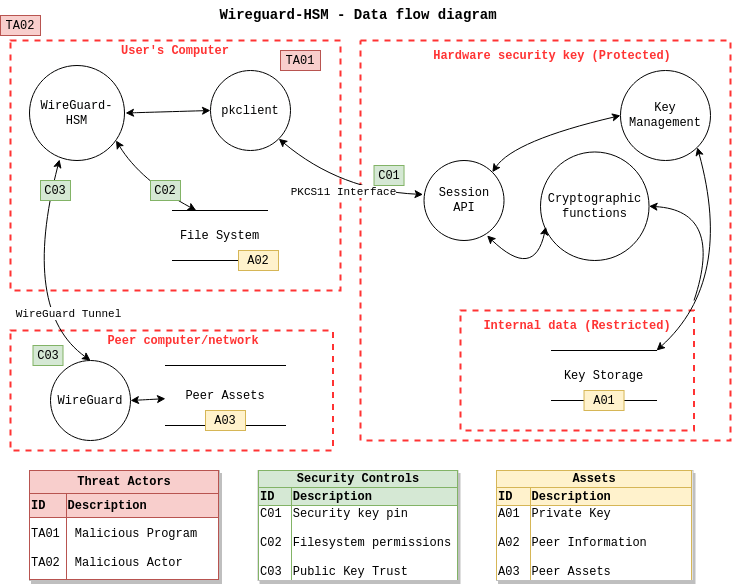
\includegraphics[width=14cm]{paper/images/WGHSM_DFD.png}
\caption{A Threat Model for WireGuard-HSM - Data Flow Diagram}
\label{fig:wg_hsm_dfd}
\end{figure}

\subsection{Assets}
The file system on Alice's computer contains the WireGuard-HSM configuration file, example in figure \ref{fig:wg_config}. 
Asset A01 is Alice's Curve25519-based long-term static private key. Asset A02 is Bob's peer information consisting of his static public key and internet address.
Asset 03 is the label for any potential assets on Bob's side of the WireGuard tunnel. Access to Bob's machine might be a highly valuable asset or Bob's network access might be the highly valuable asset. This model combines these possibilities into 'Peer Assets' for simplification.

\subsection{Security controls}
Access to asset A01 is behind two controls. First A01 is now on a physically separate system, the HSM. Alice must plug in the HSM and authenticate with a PIN, Control C01, before cryptographic operations can be performed on A01 via the PKCS\#11 interface with the session API.
File system permissions are used to protect the Peer Information, A02.
Security control C03, access to each WireGuard peer, is the pre-shared public key system implemented by WireGuard.

\subsection{Threat Actor 1}
The primary threat is TA01: a piece of malware that has gained access to Alice's computer and will search for keys in configuration files. This malware could have been delivered by acquiring a zero-day exploit or by using a known vulnerability with a piece of software running on Alice's computer. Using a known vulnerability would likely lower the cost of the attack.

\subsubsection{Insufficient permissions}
If TA01 gains access to Alice's computer and the file system permissions were not correctly set on the WireGuard-HSM configuration file, then the threat gains access to the A02: Peer Information. Loss of A02: Peer Information, may be desirable for an attacker but this does not enable an additional vulnerability in the system.
See table \ref{attack1-hsm} and \ref{attack3-hsm}.

\subsubsection{Sufficient permissions}
If C01: File system permissions, is configured properly, then TA01 will need to use an additional exploit to bypass the file system permissions and access A02, slightly increasing the cost of the attack. Loss of A02: Peer Information, may be desirable for an attacker but this does not enable an additional vulnerability in the system.
See table \ref{attack2-hsm} and \ref{attack4-hsm}.

\subsection{Threat Actor 2}
TA02 is a malicious user who gains direct or indirect access to Alice's computer. 

\subsubsection{Physical Access}
In a direct method of attack, TA02 gains physical access to Alice's computer and uses some technical or non-technical exploit to read the hard-drive. If Alice's machine uses disk-encryption then this increases the cost of the attack because a second exploit must be used to read the disk contents.
Loss of A02: Peer Information, may be desirable for an attacker but this does not enable an additional vulnerability in the system.
A01 is held on Alice's HSM not on the computer.
See table \ref{attack5-hsm} and \ref{attack6-hsm}.

If Alice left her HSM connected to her computer, then there is a risk that the threat actor could gain physical access to both Alice's computer and her HSM. Access to the HSM is protected by C01, Alice's PIN. Brute forcing HSM PIN is very unlikely because a Nitrokey Start will become blocked after three incorrect guesses and further attempts will wipe the device.

This attack could go one step further but it would require a highly-sophisticated attacker. If the attacker had knowledge of an exploit to extract the keys from the HSM, then this attack could be successful but at a decreased likelihood due to the cost of mounting a successful attack on an HSM. Information disclosure of A01 and A02 would result in loss of A03 by allowing the bypass of C03. 
See table \ref{attack8-hsm}.

\subsubsection{Social Engineering}
The indirect method of attack could be performed by TA02 using social engineering tactics, such as a phone-call or email, masquerading as someone from Alice's IT department, asking her to, in some way, disclose the contents of the WireGuard configuration file, leading to the disclosure of asset A02.

The HSM has controls in place to prevent anyone from accessing the private key, so Alice cannot be convinced to disclose it.
A successful social engineering attack could still be conceivably possible, if Alice was somehow convinced by the threat actor to give away physical possession of her HSM and PIN number, as well as the contents of the WireGuard-HSM configuration file. This represents a very high cost for a successful attack which decreases the likelihood that this weakness will be exploited by an attacker. 
See table \ref{attack9-hsm}.

\section{Vulnerabilities}
\label{hsm-vulns}
The two attacks described in HSM-ATTACK-8 and HSM-ATTACK-9 result in the same vulnerabilities in the system as described in section \ref{vulns}. These attacks require a very-high level of sophistication to carry out and come at a high-cost but it is useful to consider as many scenarios as possible.

\subsection{Attack Tables}
\begin{table}[H]
\label{attack1-hsm}
\begin{tabular}{|m{3cm}|m{.9cm}|p{27em} |}
\multicolumn{3}{l}{Potential for: Information Disclosure}                   \\
\hline
Category & Score & Rationale                                                    \\
\hline
Damage          & 1     & The public key of the peer is revealed            \\
\hline
Reproducibility & 6     & Two steps required, tooling and scripting readily available    \\
\hline
Exploitability & 5      & Exploit is available/understood, usable with only moderate skill by authenticated users or malware \\
\hline
Affected users  & 0     & There is no direct effect on any user                     \\
\hline
Discoverability & 5     & Attack may be targeted - exploited by general malware infection \\
\hline
\multicolumn{3}{l}{\textbf{Dread Score: 3.4}} 
\end{tabular}
\caption{Attack 1 - Loss of A02 after access to configuration file by using malware delivered using a known vulnerability and the configuration file permissions are incorrectly set.}
\end{table}

\begin{table}[H]
\label{attack2-hsm}
\begin{tabular}{|m{3cm}|m{.9cm}|p{27em} |}
\multicolumn{3}{l}{Potential for: Information Disclosure}                   \\
\hline
Category & Score & Rationale \\
\hline
Damage          & 1     & Loss of A01, A02, A03. DoS for a single user possible            \\
\hline
Reproducibility & 5     & Three steps required, tooling and scripting readily available    \\
\hline
Exploitability & 5      & Exploit is available/understood, usable with only moderate skill by authenticated users or malware \\
\hline
Affected users  & 0     & At least two users are affected                      \\
\hline
Discoverability & 4     & Attack may be targeted - exploited by general malware infection \\
\hline
\multicolumn{3}{l}{\textbf{Dread Score: 3.0}} 
\end{tabular}
\caption{Attack 2 - Loss of A02 after access to configuration file by using malware delivered using a known vulnerability and the configuration file permissions are correctly set.}
\end{table}

\begin{table}[H]
\label{attack3-hsm}
\begin{tabular}{|m{3cm}|m{.9cm}|p{27em} |}
\multicolumn{3}{l}{Potential for: Information Disclosure}                   \\
\hline
Category & Score & Rationale \\
\hline
Damage          & 1     & Loss of A01, A02, A03. DoS for a single user possible            \\
\hline
Reproducibility & 4     & Two steps required, tooling and scripting readily available    \\
\hline
Exploitability & 4      & Advanced techniques required. General malware infection would have unimpeded access to access assets  \\
\hline
Affected users  & 0     & At least two users are affected                      \\
\hline
Discoverability & 4     & Attack may be targeted - exploited by advanced malware \\
\hline
\multicolumn{3}{l}{\textbf{Dread Score: 2.6}} 
\end{tabular}
\caption{Attack 3 - Loss of A02 after access to configuration file by using malware delivered using a zero-day exploit and the configuration file permissions are incorrectly set.}
\end{table}

\begin{table}[H]
\label{attack4-hsm}
\begin{tabular}{|m{3cm}|m{.9cm}|p{27em} |}
\multicolumn{3}{l}{Potential for: Information Disclosure}                   \\
\hline
Category & Score & Rationale \\
\hline
Damage          & 1     & Loss of A01, A02, A03. DoS for a single user possible            \\
\hline
Reproducibility & 3     & Two steps required, tooling and scripting readily available    \\
\hline
Exploitability & 3      & Advanced techniques required. General malware infection would have unimpeded access to access assets  \\
\hline
Affected users  & 0     & At least two users are affected                      \\
\hline
Discoverability & 3     & Attack may be targeted - exploited by advanced malware \\
\hline
\multicolumn{3}{l}{\textbf{Dread Score: 2.0}} 
\end{tabular}
\caption{Attack 4 - Loss of A02 after access to configuration file by using malware delivered using a zero-day exploit and the configuration file permissions are correctly set.}
\end{table}

\begin{table}[H]
\label{attack5-hsm}
\begin{tabular}{|m{3cm}|m{.9cm}|p{27em} |}
\multicolumn{3}{l}{Potential for: Information Disclosure}                   \\
\hline
Category & Score & Rationale \\
\hline
Damage          & 1     & Loss of A01, A02, A03. DoS for a single user possible            \\
\hline
Reproducibility & 4     & Two steps required. Attacker must gain physical access to the computer     \\
\hline
Exploitability & 7      & Exploit is understood, usable by unskilled attacker \\
\hline
Affected users  & 0     & At least two users are affected                      \\
\hline
Discoverability & 3     & Attack must be targeted to user \\
\hline
\multicolumn{3}{l}{\textbf{Dread Score: 3.0}} 
\end{tabular}
\caption{Attack 5 - Loss of A02 after access to configuration file by using physical access to unprotected machine. }
\end{table}

\begin{table}[H]
\label{attack6-hsm}
\begin{tabular}{|m{3cm}|m{.9cm}|p{27em} |}
\multicolumn{3}{l}{Potential for: Information Disclosure}                   \\
\hline
Category & Score & Rationale \\
\hline
Damage          & 1     & Loss of A01, A02, A03. DoS for a single user possible            \\
\hline
Reproducibility & 4     & Two steps required. Attacker must gain physical access to the computer     \\
\hline
Exploitability & 5      & Exploit is understood, usable by moderately skilled attacker  \\
\hline
Affected users  & 0     & At least two users are affected                      \\
\hline
Discoverability & 3     & Attack must be targeted to user \\
\hline
\multicolumn{3}{l}{\textbf{Dread Score: 2.6}} 
\end{tabular}
\caption{Attack 6 - Loss of A02 after access to configuration file by using physical access to a protected machine. }
\end{table}

\begin{table}[H]
\label{attack7-hsm}
\begin{tabular}{|m{3cm}|m{.9cm}|p{27em} |}
\multicolumn{3}{l}{Potential for: Information Disclosure}                   \\
\hline
Category & Score & Rationale \\
\hline
Damage          & 1     & Loss of A01, A02, A03. DoS for a single user possible            \\
\hline
Reproducibility & 5     & Two steps required. Attacker must find and convince user to disclose contents of configuration file    \\
\hline
Exploitability & 5      & Little technical knowledge is required but trust or deception must be used   \\
\hline
Affected users  & 0     & At least two users are affected                      \\
\hline
Discoverability & 9     & Weakness is is well understood  \\
\hline
\multicolumn{3}{l}{\textbf{Dread Score: 4}} 
\end{tabular}
\caption{Attack 7 - Loss of A02 after access to configuration file is gained by social engineering}
\end{table}

\begin{table}[H]
\label{attack8-hsm}
\begin{tabular}{|m{3cm}|m{.9cm}|p{27em} |}
\multicolumn{3}{l}{Potential for: Information Disclosure, Spoofing, DoS}                   \\
\hline
Category & Score & Rationale \\
\hline
Damage          & 9     & Loss of A01, A02, A03. DoS for a single user possible            \\
\hline
Reproducibility & 1     & Very difficult to reproduce, may be possible once or twice  \\
\hline
Exploitability & 1      & Extreme level of technical exploitation needed. Possibly a Nation-State actor  \\
\hline
Affected users  & 5     & At least two users are affected                      \\
\hline
Discoverability & 3     & Intimate knowledge of the target would be needed to successfully target user \\
\hline
\multicolumn{3}{l}{\textbf{Dread Score: 3.8}} 
\end{tabular}
\caption{Attack 8 - Loss of A01 and A02 after TA02 convinces Alice to give away her HSM and disclose the contents of her WireGuard configuration file. }
\end{table}

\begin{table}[H]
\label{attack9-hsm}
\begin{tabular}{|m{3cm}|m{.9cm}|p{27em} |}
\multicolumn{3}{l}{Potential for: Information Disclosure, Spoofing, DoS}                   \\
\hline
Category & Score & Rationale \\
\hline
Damage          & 9     & Loss of A01, A02, A03. DoS for a single user possible            \\
\hline
Reproducibility & 0     & Very hard or impossible. The vulnerability is unstable and statistically unlikely to be reliably exploited   \\
\hline
Exploitability & 1      & Extreme level of technical exploitation needed. Possibly a Nation-State actor   \\
\hline
Affected users  & 5     & At least two users are affected                      \\
\hline
Discoverability & 1     & Weakness is currently unknown but a targeted attacker with knowledge of the system is possible   \\
\hline
\multicolumn{3}{l}{\textbf{Dread Score: 3.2}} 
\end{tabular}
\caption{Attack 9 - Loss of A01 and A02 after TA02 breaks into the machine and uses sophisticated methods to extract the private key from the HSM }
\end{table}


\chapter{Performance and code evaluation}
\section{Performance Analysis}

\label{performance}
WireGuard-HSM's use of a USB-connected HSM means a small part of its functionality is embedded inside a much less powerful computer than the computer running the WireGuard-HSM program. I wanted to see what performance impacts this design might introduce to the system. 

In order to benchmark the performance of the implementations, I added a timing function that saves the current time at the beginning of the sharedSecret() function in WireGuard and DeriveNoise() in pkclient. WireGuard-HSM will still make use of sharedSecret() for ephemeral key operations.
See section \ref{fig:keyflow} for more details on when sharedSecret() is called vs DeriveNoise().

The benchmarks were run on two computers connected via a local Gigabit Ethernet connection. 
WireGuard-HSM ran on a desktop PC running Ubuntu 21.10 configured with an AMD Ryzen 5 2600 CPU @ 3.4GHz nominal speed and 64 GB DDR4 ram. 

The peer computer ran an unmodified WireGuard client included with Ubuntu 21.10 on a machine with an Intel core i5-4590 CPU @ 3.30GHz nominal speed and 16 GB DDR3 ram.  

Each function test was run until 32 function calls had been recorded for the target function, labeled DeriveNoise() for the security key and DeriveSoftware() for the default WireGuard software derive function.
Each test was run 3 times and the results were compiled together for an total of 96 data points for each function. A descriptive statistic analysis performed on the resulting data set.

\begin{figure}
\centering
\begin{minipage}{.5\textwidth}
  \centering
  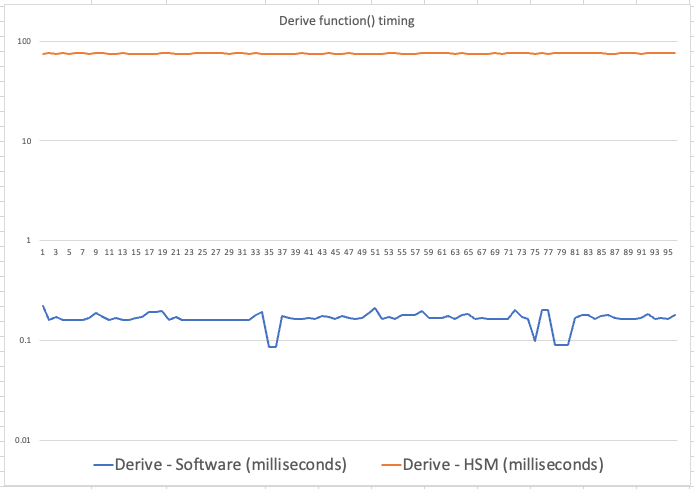
\includegraphics[width=1\linewidth]{paper/images/deriveFunctiongraph.png}
  \caption{Execution Time for DeriveNoise() and softwareDerive()}
  \label{fig:funcTimeGraph}
\end{minipage}%
\begin{minipage}{.5\textwidth}
  \centering
  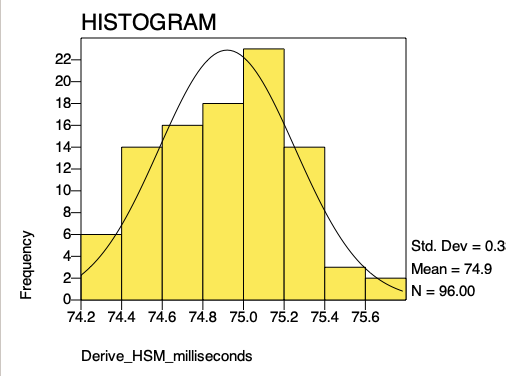
\includegraphics[width=1\linewidth]{paper/images/DeriveNoise freq.png}
  \caption{Histogram of DeriveNoise Execution Time in Milliseconds}
  \label{fig:hsmTimeGraph}
\end{minipage}
\end{figure}

The mean execution time for DeriveHSM() is 74.9 milliseconds and the standard deviation is 0.3 milliseconds. The variance across all data points is .11 milliseconds. 

The mean execution time for softwareDerive() is 0.17 milliseconds and the standard deviation is 0.02 milliseconds. The variance across all data points was too small to be significant.

\section{Code size}
\label{loc}
The total number of lines of code (LOC) changed in WireGuard-HSM when compared to WireGuard-Go is currently 104. If I only count lines of code changed to the core WireGuard protocol files, then the count drops to only 44 LOC changes. A very easy number of changes to audit and understand.

The Pkclient module is 230 LOC in total.

\chapter {Discussion of Results}
Here we will discuss the results from the previous sections.

\section{Threat Model Comparison}
Attacks 1-7 are are shared by both WireGuard and WireGuard-HSM. The impact of Attacks 1-7 on WireGuard-HSM have almost no 'damage', according to the DREAD calculations. For WireGuard-HSM, the vulnerabilities identified for WireGuard in section \ref{vulns} are successfully mitigated. Even though the system still has a weakness that can be used to expose the public key of the peer, WireGuard-HSM manages to maintains the confidentiality of the users' private key.

Table \ref{tab:DREAD_AVG} shows the summary of the shared attacks for both systems.

\begin{table}[h!]
  \begin{center}
    \caption{DREAD results for shared attacks}
    \label{tab:DREAD_AVG}
    \begin{tabular}{c|c|c}
      \textbf{Attack \#} & \textbf{WireGuard ref impl.} & \textbf{WireGuard-HSM}\\
      \hline
      1 & 6.0 & 3.4\\
      2 & 5.6 & 3.0\\
      3 & 5.2 & 2.6\\
      4 & 4.6 & 2.0\\
      5 & 5.6 & 3.0\\
      6 & 5.2 & 2.6\\
      7 & 6.6 & 4.0\\
    \hline
    Avg & 5.5 & 2.9\\
    $\sigma$ &  0.59 & 0.59\\
    $\sigma^2$ &  0.35 & 0.35\\
    \end{tabular}
  \end{center}
\end{table}

If we subtract WireGuard-HSM's average DREAD score from WireGuard's average DREAD score, then WireGuard-HSM reduces the average DREAD score of these shared attack scenarios by 2.6 points.

In section \ref{hsm-vulns} we considered two additional attacks for WireGuard-HSM, HSM-ATTACK-8 and HSM-ATTACK-9. 
These two attacks have an average DREAD rating of 3.5. Their risk is low but it demonstrates that no security solution is perfect. HSM vulnerabilities may be found and users must be informed about the dangers social engineering attacks.
A successful attack would also lead to a spoofing and DoS vulnerability in WireGuard-HSM. Since the reproducibility and exploitability of those attacks is very low, I consider it an acceptable risk for the benefits to security that WireGuard-HSM demonstraighted in attacks 1-7.


\subsection{Attack Surface}
The threat model analysis of WireGuard-HSM in section \ref{wg-hsm-analysis} shows that any attack against the system, where the attacker can read the sensitive configuration file, will no-longer result in the loss of the user's private key because of how WireGuard-HSM keeps sensitive data confidential. Since the confidentiality of the private-key is maintained the previous vulnerabilities in WireGuard a no longer exposed. This demonstrates that WireGuard-HSM successfully reduces in the the attack surface.

The number of lines of code changed in WireGuard-HSM to the original program was minimal, making an audit of the code an easy task.

\subsection{performance}
The performance analysis shows the impact of using the Nitrokey Start, in  WireGuard-HSM is less than a tenth of a second per-handshake. If the typical use-case for WireGuard-HSM is two users establishing a session over the internet, then there should be no noticeable delay.

\subsection{Compatibility}
All tests of WireGuard-HSM were carried out by establishing a session with a peer running the reference implementation of WireGuard using the Linux kernel module. This successfully demonstrates the compatibility of WireGuard-HSM.

\section {Limitations}
In this section I will discuss the limitations of my project in regards to the completeness of the evaluation and the limitations of the project implementation itself. Significant time was spent to get the technical implementation of the project working, so I will discuss what improvements I would like to see, if I had more time to complete the evaluation of the entire system.

\subsection{Formal Analysis}
A formal analysis was identified as an aspirational goal for this project. If I had more time, I would perform a formal analysis of the security properties of WireGuard-HSM. The original WireGuard protocol has been verified using the Tamarin prover\cite{donenfeld_formal_2018}, so I would also like to define and verify WireGuard-HSM in the Tamarin prover to create a symbolic model of the system. This would further demonstrate how the security properties of WireGuard-HSM are correctly maintained.

\subsection{Mobile Operating Systems}
I had initially planned to support mobile operating systems such as a smart-phones. Users can easily use security keys with mobile operating systems but due to technical requirements of the WireGuard protocol, a WireGuard-HSM user would have to leave their security key constantly connected
or after 2\textsuperscript{60} messages are exchanged. This could be avoided by having users modify their WireGuard client and peer defaults to a much longer timeout for re-key, but this seems like a burdensome approach and it may not be possible for the client to request a modification of peer settings.

\subsection{HSM limitations}
Adding a physical piece of hardware like an HSM into a software system adds complexity and decreases the user-convenience of the system. The correct port-type must be available on the user's machine. HSMs can be lost, stolen, break, or wear-out. By design, the private keys on the HSM cannot be copied, so if the HSM breaks, the user will need to purchase a new one and manually go through the out of band key exchange process with a new public key.

\chapter {Future work and conclusion}

\section {Future Work}
There are several areas of improvement for WireGuard-HSM that have been identified over the course of implementing and evaluating the system. 

\subsection{Pin handling}
When WireGuard-HSM starts, it prompts the user on the command-line for the PIN to the slot on the HSM. 
This prompt is easy to miss and wouldn't work very well if WireGuard-HSM was implemented as a kernel module. A better approach would be to have the prompt implemented as a system-dialog window, that appears over any existing windows, making very simple for the user to omit the pin and only enter it when using WireGuard-HSM. Finding a Go-module that opens window dialogues and supports multiple operating system was deemed out of scope for this project but it will be my next addition to the program since it would increase the ease-of-use for the program. 
 
\subsection{Security Key Diversity}
Hardware security-key support for curve25519 and specifically X25519 is, as of writing, very limited. Nitrokey 3 is planned to support X25519 but the hardware is still not in mass production. I would like to see biometric hardware-keys with X25519 support, this would add an additional layer of security to our model as it further authenticates the user. As of writing, I could find no planned development for such a key. Many hardware-security keys have introduced support for near-field-communication (NFC) which makes using them with mobile devices almost seamless. Having a security-key with Curve25519 support, would make integrating WireGuard-HSM with mobiles devices easier and put less burden on the user. 

\subsection{Kernel-Mode Support}
WireGuard-HSM is written using the Go language version of WireGuard but a kernel-mode version would be more practical to most users. The Go-version of WireGuard warns users on start-up that if they are on a supported operating system, the kernel version has better support and offers better performance. The main challenge in writing the kernel mode version will be the PKCS\#11 integration and handling user interaction between a kernel module. A small program like pkclient that handled the PKCS\#11 integration and user prompts would be a good first step in expanding the functionality.

\subsection{Biometric Authentication}
It would be desirable for this project to use a biometric security key; for example, a security key that uses a small fingerprint reader to authenticate the user. A biometric security key with X25519 support is not yet offered together but they exist in independent implementations, for example Yubico sells a security key that has fingerprint reader needed for user authentication\cite{yubico_yubikey_2022}. 

\section{Conclusion}
WireGuard-HSM helps mitigate the impact of weaknesses in the reference implementation of WireGuard by increasing the confidentiality of the user's private key. WireGuard-HSM successfully mitigates both a spoofing and DoS vulnerability found during a threat model analysis of WireGuard.
WireGuard-HSM's performance impact is negligible and should be unnoticeable to users.
This project offers a compelling example for more system designers to integrate a Hardware Security Module with Curve25519 support, into their product.


\bibliographystyle{plain}
\bibliography{references}

\appendix



\begin{table}[ht]
\begin{tabular}{llllll}
\begin{tabular}[c]{@{}l@{}}Test 1\\ HSM\end{tabular} & \begin{tabular}[c]{@{}l@{}}Test 1\\ Software\end{tabular} & \begin{tabular}[c]{@{}l@{}}Test 2\\ HSM\end{tabular} & \begin{tabular}[c]{@{}l@{}}Test 2\\ Software\end{tabular} & \begin{tabular}[c]{@{}l@{}}Test 3\\ HSM\end{tabular} & \begin{tabular}[c]{@{}l@{}}Test 3\\ Software\end{tabular} \\
0.074625 & 0.000222 & 0.075195 & 0.00018 & 0.074567 & 0.000183 \\
0.075144 & 0.00016 & 0.074526 & 0.000195 & 0.074839 & 0.000165 \\
0.074853 & 0.00017 & 0.074719 & 0.000086 & 0.074444 & 0.000167 \\
0.075121 & 0.000159 & 0.074356 & 0.000085 & 0.074543 & 0.000165 \\
0.074688 & 0.000159 & 0.074818 & 0.000175 & 0.075265 & 0.000165 \\
0.075275 & 0.00016 & 0.07454 & 0.000169 & 0.074292 & 0.000165 \\
0.075482 & 0.00016 & 0.074292 & 0.000165 & 0.074961 & 0.000164 \\
0.07468 & 0.000168 & 0.074977 & 0.000165 & 0.075102 & 0.000201 \\
0.075142 & 0.000188 & 0.074907 & 0.000166 & 0.074971 & 0.000172 \\
0.075259 & 0.000172 & 0.074395 & 0.000165 & 0.075421 & 0.000165 \\
0.074472 & 0.000161 & 0.074577 & 0.000177 & 0.074457 & 0.000098 \\
0.074809 & 0.000168 & 0.075213 & 0.00017 & 0.075326 & 0.000202 \\
0.075128 & 0.00016 & 0.074541 & 0.000164 & 0.074649 & 0.0002 \\
0.074773 & 0.00016 & 0.074462 & 0.000176 & 0.075058 & 0.000091 \\
0.074744 & 0.000167 & 0.07527 & 0.000169 & 0.075316 & 0.000091 \\
0.074798 & 0.000171 & 0.074572 & 0.000165 & 0.07518 & 0.000091 \\
0.074298 & 0.000195 & 0.07461 & 0.000168 & 0.07516 & 0.000166 \\
0.074475 & 0.000195 & 0.074765 & 0.000189 & 0.075529 & 0.00018 \\
0.075175 & 0.000196 & 0.074652 & 0.000212 & 0.075783 & 0.000179 \\
0.075066 & 0.00016 & 0.074647 & 0.000165 & 0.075094 & 0.000165 \\
0.074905 & 0.000171 & 0.075391 & 0.000171 & 0.075116 & 0.000176 \\
0.074811 & 0.000161 & 0.075196 & 0.000165 & 0.074684 & 0.000179 \\
0.074932 & 0.00016 & 0.074861 & 0.000179 & 0.074531 & 0.000169 \\
0.074969 & 0.00016 & 0.074525 & 0.000178 & 0.075348 & 0.000165 \\
0.075188 & 0.000159 & 0.074627 & 0.000178 & 0.075074 & 0.000165 \\
0.075258 & 0.00016 & 0.074947 & 0.000199 & 0.075354 & 0.000165 \\
0.075104 & 0.00016 & 0.075131 & 0.000168 & 0.074877 & 0.000166 \\
0.075275 & 0.000159 & 0.07513 & 0.000167 & 0.074998 & 0.000183 \\
0.074619 & 0.000161 & 0.074947 & 0.000166 & 0.075389 & 0.000165 \\
0.075087 & 0.00016 & 0.075004 & 0.000175 & 0.075642 & 0.000169 \\
0.075038 & 0.000159 & 0.074628 & 0.000164 & 0.075108 & 0.000165 \\
0.074364 & 0.00016 & 0.074966 & 0.00018 & 0.075239 & 0.000181
\end{tabular}
\end{table}
\end{document}
